\documentclass[12pt,a4paper]{article}  % Déclare la classe du document.

%  ------------------------------------------  Modules usuels  --------------------------------------
%  --------------------------------------------------------------------------------------------------------

\usepackage{amsmath} 	
\usepackage{amssymb} 
\usepackage{listings}         
\usepackage{numprint} 
\usepackage{pifont}

%  --------------------------------------------------------------------------------------------------------
% ----------------------  packages pour fontes et caractères spéciaux  ---------------------
%  --------------------------------------------------------------------------------------------------------

\usepackage{eurosym}   
\usepackage{amsfonts}   
\usepackage{amstext}       
\usepackage{amsfonts}	
\usepackage{mathrsfs}	 

\usepackage{pstricks,pst-all,pstricks-add,pst-tree,pst-node,pst-3dplot}

%------------------------------------------------------------------------------------------------------
%  --------------------------  Francisation et gestion des caractères sous mac --------------------------------------------------------------------------------------------------------

\usepackage[francais]{babel}   
\usepackage[utf8]{inputenc}
\usepackage[OT1,T1]{fontenc} 
%  --------------------------------------------------------------------------------------------------------
% ------------------------------------Packages  de  mise en page ---------------------------
%--------------------------------------------------------------------------------------------------------

\usepackage{fancyhdr}	% en-têtes et pieds de pages
\usepackage{amsfonts}

 \usepackage{multicol} % permet l'utilisation du multicolonnage dans le texte. La syntaxe est \begin{multicols}{nb de colonnes}    ......  \end{multicols}
 
\usepackage{calc}            % permet de faire un minimum de calcul sur les arguments des commandes et macros (utilisé dans la def de l'environnement preuve )
\usepackage{epic}            % extension et simplification de  l'environnement picture
\usepackage{graphicx}    % permet d'inclure des graphique externe dans un document
\usepackage{variations}   % permet d'obtenir de joli tableau de variations
\usepackage{enumerate}  %permet de faire des listes personnalisées
\usepackage{arydshln}     %permet d'avoir des lignes en pointillés
\usepackage{framed}  
\usepackage{multido} 


%  --------------------------------------  MACROS USUELLES  ----------------------------------------

\newcommand{\R}{\mathbb{R}} 
\newcommand{\N}{\mathbb{N}} 
\newcommand{\D}{\mathbb{D}} 
\newcommand{\Z}{\mathbb{Z}} 
\newcommand{\Q}{\mathbb{Q}} 
\newcommand{\C}{\mathbb{C}} 

%  -------------------------------------  MACROS SPECIFIQUES ------------------------------------


\newcommand{\raisedrule}[2][0em]{\leaders\hbox{\rule[#1]{1pt}{#2}}\hfill}


\newcounter{numexo}

\setcounter{numexo}{1}

\newcommand{\exercice}[1]{\vskip 0.6cm\noindent\rule[+2pt]{1cm}{0.5pt}\ {\large\bf \ Exercice \thenumexo {  #1 }}\raisedrule[+2pt]{0.5pt}\null\addtocounter{numexo}{1}\par\vskip 0,4cm}


\newcommand{\lignes}[1]{
\setlength{\unitlength}{1mm}
\vskip 0,4cm\noindent
\multido{\i=0+1}{#1}{%
     \noindent
     \begin{picture}(150,5)
     \linethickness{0,005mm}
     \put(-5,0){\dashline{1}(175,5)(5,5)}
     \end{picture}\vskip 0,001cm
     }
\vskip 0cm
}




% ----------------------------------------- FORMAT DE PAGE  -----------------------------------------

\usepackage[left = 1.3cm,
	 	      right = 1.3cm,
		      top = 1.7cm,
		      headsep = 8mm,
		      bottom = 1.7cm,
		      headheight = 14.2 pt
		      ]{geometry}

\setlength{\parindent}{0mm}


\everymath{\displaystyle} 
\renewcommand{\thesection}{\Roman{section}} 
\author{}
\title{}
\date{}
\pagestyle{fancy}

 
\lhead{1ère - spécialité maths} 


\rhead{DS n$^{\circ}$5 - 27/01/21}		


\fancyfoot[C]{} 
\fancyfoot[L]{} 
\fancyfoot[R]{} 

\lstset{language=Python}  

\lstset{frame = single
framerule = 1pt
showspaces = false,
showstringspaces = false,
numbers=left, numberstyle=\tiny}

% ----------------------------------------- correction  -----------------------------------------
\usepackage[most,skins,breakable]{tcolorbox}
\usepackage{enumitem}

\newcommand{\corr}[1]{\fcolorbox{red}{yellow!30}{#1}}

\newtcolorbox{corrBox}{enhanced,boxrule=1pt,nobeforeafter,boxsep=0pt,left=\fboxsep,right=\fboxsep,colback=yellow!30,colframe=red!75!black}

\newlist{enumMet}{enumerate}{2}
\setlist[enumMet,1]{label=\arabic*), font=\bf\color{blue!75!black}}
\setlist[enumMet,2]{label=\alph*), font=\bf\color{blue!75!black}}


\begin{document}
\graphicspath{{images/}}

\begin{center}

\fbox{\LARGE{\rule{0.5cm}{0pt}\rule[-0.25cm]{0pt}{0.9cm} Devoir Surveillé N$^{\circ}$5 - Produit scalaire et nombre dérivé	\rule{0.5cm}{0pt}}}
\end{center}


\begin{center}\textbf{2h - Calculatrice autorisée - Barème indicatif}\end{center}

%\begin{center}\textbf{Les élèves avec un tier-temps ne traitent pas les questions avec  le symbole \ding{46}}\end{center}

\begin{center}
%On veillera à ENCADRER ses résultats et soigner sa copie.\\
Les résultats doivent être justifiés par des calculs (au moins 1 étape intermédiaire).
\end{center}
\vspace{.05cm} 

\vspace{-0.3cm}
\exercice{ - définition du produit scalaire - ( 1 point )}
On considère 3 points $A, B$ et $C .$ Dans chacun des cas suivants, calculer $\overrightarrow{A B} \cdot \overrightarrow{A C}$ ( on donnera la valeur exacte).
\begin{multicols}{2}
\begin{enumMet}
    \item $A B=3, A C=7$ et $\widehat{A B C}=\dfrac{\pi}{3}$
    \item $A B=4, A C=9$ et $\widehat{A B C}=\dfrac{\pi}{4}$
\end{enumMet}
\end{multicols}


\exercice{ - projection orthogonale - ( 1,5 points )}

On considère un carré ABCD de côté 5.\\
Calculer $\overrightarrow{A B} \cdot \overrightarrow{A C}, \overrightarrow{C A} \cdot \overrightarrow{C D}$ et $\overrightarrow{D C} \cdot \overrightarrow{D A}$

\exercice{ - produit scalaire dans un triangle - ( 1 point )}

Soit un triangle $\mathrm{ABC}$ de longueur $\mathrm{AB}=5, \mathrm{AC}=7$ et $\mathrm{BC}=10$\\
Calculer le produit scalaire $\overrightarrow{B A} \cdot \overrightarrow{B C}$

\exercice{ - produit scalaire dans un repère - ( 2 points )}

Soit les points $A(3 ; 3), B(8 ; 6)$ et $C(13 ; 3)$
\begin{enumMet}
    \item Calculer le produit scalaire $\overrightarrow{B A} \cdot \overrightarrow{B C}$
    \item Que peut-on en conclure pour le triangle ABC?
\end{enumMet}


\exercice{ - Au golf - ( 1,5 points )}
\begin{minipage}[c]{.6\linewidth}
Sur un green de golf, trois positions de la balle sont repérées en $\mathrm{M},$ N et P sur le schéma ci-contre. Le triangle MNP est tel que MN=8, $\mathrm{MP}=5$ et $\widehat{M}=53^{\circ}$.\\
Calculer la valeur exacte de NP, puis son arrondi à 0,1 près.
\end{minipage}
\hfill
\begin{minipage}[c]{.35\linewidth}
\begin{center}
   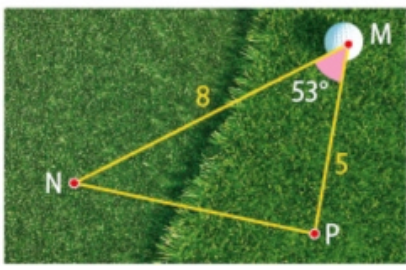
\includegraphics[scale=0.8]{1.05.DS-IMG-01} 
\end{center}

\end{minipage}

\exercice{ - équation cartésienne - ( 1 point )}

Déterminer dans le cas ci-dessous, une équation cartésienne de la droite D qui passe par le point $A$ et qui a pour vecteur normal le vecteur $\vec{n}$\\
$A(3 ; 4)$ et $\vec{n}\left(\begin{array}{c}-3 \\ 5\end{array}\right)$

\newpage

\exercice{ - nombre dérivé - ( 3 points )}
Sur chacun des deux graphiques suivants sont représentées la courbe $C_{f}$ d'une fonction $f$ dérivable en a et sa tangente T au point d'abscisses Dans chacun des cas, déterminer par lecture graphique les nombres $a, f(a)$ et $f^{\prime}(a)$
\begin{center}
    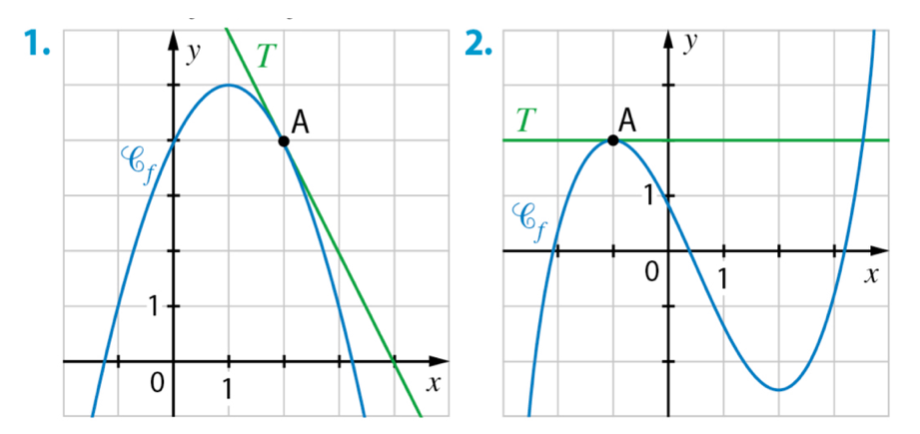
\includegraphics[scale=0.8]{1.05.DS-IMG-02}
\end{center}

\exercice{ - nombre dérivé - ( 2 points )}
Une fonction $f$, dérivable sur $\mathbb{R}$, admet la représentation graphique $\mathscr{b}_{f}$ ci-dessous. La droite (AB) est tangente à $\mathscr{b}_{f}$ au point $A$ d'abscisse -2
\begin{enumMet}
    \item déterminer par la méthode de votre choix l'équation réduite de la droite $(AB)$
    \item en déduire le nombre dérivé de $f$ en $-2$. 
\end{enumMet}
\begin{center}
    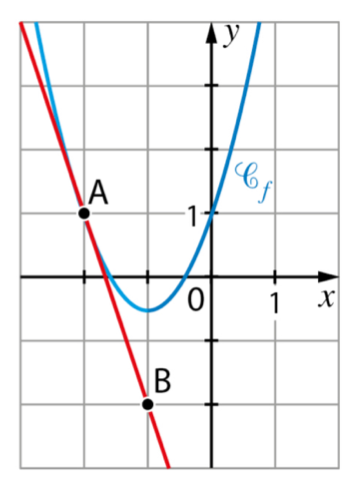
\includegraphics[scale=0.8]{1.05.DS-IMG-03}
\end{center}

\exercice{ - dérivabilité - ( 2 points )}

Soit $f$ la fonction définie sur $R \operatorname{par} f(x)=2 x^{2}-2 x+5$\\
Montrer que la fonction f est dérivable pour $\mathrm{x}=2$ et calculer $f^{\prime}(2)$

\exercice{ - dérivabilité - ( 2 points )}
Soit f la fonction définie sur $] 2 ;+\infty\left[\operatorname{par} f(x)=\frac{1}{x-2}\right.$\\
Montrer que la fonction f est dérivable pour $x=3$ et calculer $f^{\prime}(3)$

\exercice{ - dérivabilité - ( 4 points )}
On considère la courbe représentative $C_{f}$ de la fonction $f$ définie par $f(x)=x^{2}-3 x+1$ et dérivable sur $\mathbb{R}$. Soient $D$ le point de $C_{f}$ d'abscisse 3 et $\mathrm{d}$ la tangente en $\mathrm{D}$ à la courbe $C_{f}$
\begin{center}
    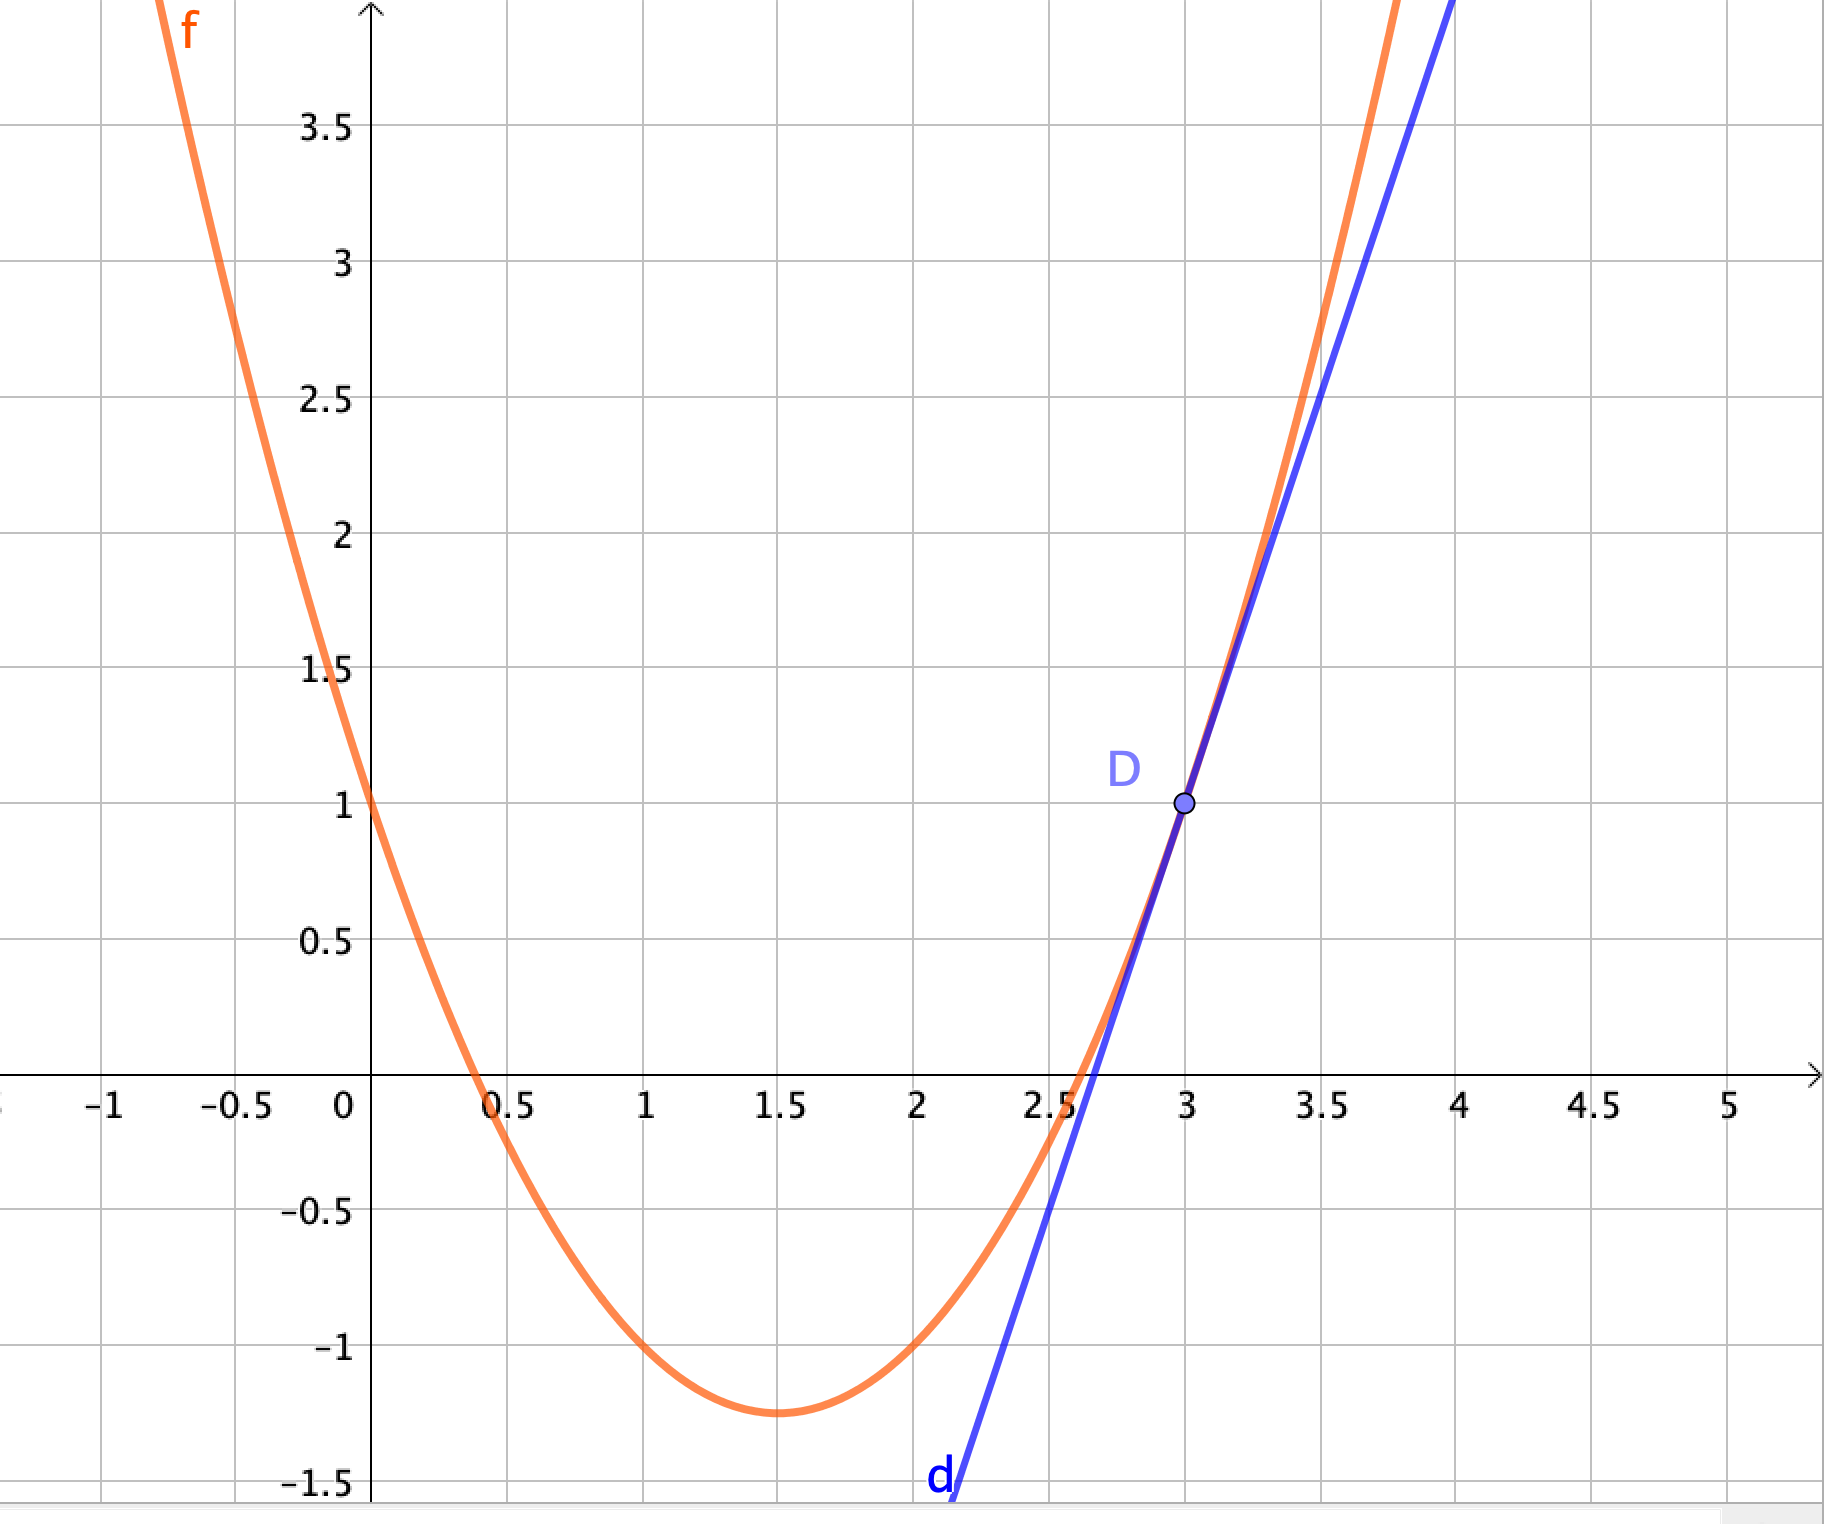
\includegraphics[scale=0.5]{1.05.DS-IMG-04}
\end{center}
\begin{enumMet}
    \item Montrer que l'équation réduite de la tangente $d$ est $y=3x-8$.
    \item Étudier la position relative de la courbe $C_{f}$ par rapport à sa tangente $d$. On pourra éventuelle ment utiliser la calculatrice pour déterminer le signe d'un trinôme.
\end{enumMet}
\end{document}

